


\subsection{Enjeux industriels et économiques}

%% A deplacer dans CONTRAINTES  
De façon plus générale, les enjeux industriels peuvent varier selon les domaines. Ceci étant dit on peut nommer points principaux, qui sont ceux que l'on va tenter de prendre en considération dans cette étude. La première d'entre elle est l'imposition de capacités de déploiement rapides (\textit{"Time-to-market"} réduit). Les itérations entre générations demandent des coûts de développement les moins importants possibles. Cela permet des cycles courts et réactifs qui s'adaptent aux évolutions technologiques. Cette contrainte industrielle est structurante sur les choix de conception, ce qui nous ramène souvent au principe "KISS", i.e. "Keep It Safe and Simple" dans notre cas. C'est une philosophie que j'ai souhaité maintenir le long de cette thèse afin de tenter une approche un peu différente des principales recherches actuelles qui tentent souvent d'aller dans des niveaux de détails toujours plus précis et complexes pour répondre aux difficultés technologiques. Comme on le verra plus tard, il existe ainsi des solutions très sophistiquées qui donnent de bons résultats théoriques, mais qui ne se sont pas généralisés dans un contexte industriel. Les questions de complexité d'implémentation et simplicité de maintenance dans un cas réel semblent donc relativement déterminantes pour mesurer la pertinence d'une nouvelle contribution à la sûreté des systèmes embarqués.

On pourra mentionner aussi des contraintes spatiales. Les systèmes embarqués ont une forte tendance à la miniaturisation pour des enjeux multiples. Cela permet une réduction de poids, essentiel pour des raisons évidents pour tous les systèmes volants (avions, drones...) mais aussi d'encombrement pour des domaines comme l'automobile, le ferroviaire qui doivent en toute circonstance rester dans des dimensions standards. Cette contrainte se fait beaucoup sentir avec l'arrivée des voitures autonomes par exemple, où les premiers prototypes 


Au regard de ces enjeux et de la connectivité qui arrive dans les systèmes, l'évolution future naturelle est de réduire le nombre de calculateurs embarqué, en passant d'un grand nombre d'unités de calcul à une quantité limitée de "supercalculateurs", qui vont agréger différentes tâches. On passe de cette façon d'un système distribué à un système fédéré basé sur des calculateurs primaires accompagnés de processeurs satellites qui gèrent le strict nécessaire à hauteur des différents capteurs/actionneurs.  Cela permet de réduire les coûts et l'encombrement, qui va diminuer par la même occasion la quantité de câblages requis. Ce type d'architecture va faciliter l'évolutivité qui sera donc bien plus axée sur des mises à jour logicielles sans toucher au matériel. La connectivité permettant le concept du véhicule \textit{"as-a-service"}, qui va pouvoir évoluer et se mettre à jour régulièrement à distance (\textit{Over-the-Air Updates}). 

%%	l'évolution future naturelle est de réduire le nombre de calculateurs embarqué, en passant d'un grand nombre d'unités de calcul à une quantité limitée de "super calculateurs", qui vont agréger différentes tâches. On passe de cette façon d'un système distribué à un système fédéré basé sur des calculateurs .  Là où ce type d'architecture va permettre de faciliter l'évolutivité, réduire les coûts et l'encombrement, vont apparaître d'autres problématiques auxquelles nous allons nous intéresser.

%%	Historiquement, les calculateurs embarqués étaient conçus de manière \emph{ad hoc} : le hardware et le software étaient intimement liés. Cela a conduit à un nombre de calculateurs très important, chaque calculateur apportant sa fonctionnalité. On a donc actuellement une architecture avec un grand nombre d'ECU (Electronic Control Unit). On peut noter trois principales propriétés des systèmes embarqués automobiles :
%\begin{itemize}
%	\item Les ECU sont \emph{inter-connectés}, ils communiquent les uns avec les autres,
%	\item Les fonctions et services sont intégrés dans des sous-systèmes complexes. Ainsi un sous-système inclut divers fonctionnalités,
%	\item Les fonctions sont \emph{distribuées} sur plusieurs calculateurs. Certaines fonctions peuvent être hébergées par plusieurs micro-contrôleurs.
%\end{itemize} 
%Ce type d'architecture présentée ci-dessus a des inconvénients évidents en terme d'évolutivité du système et de temps de développement. A chaque changement de support physique (micro-contrôleur) le logiciel doit passer par un nouveau stade de développement plus ou moins conséquent. Inversement, une mise à jour du logiciel va demander une prise en compte du hardware. Cela augmente donc les temps et les coûts de développement.

\section{Enjeux des Architectures Logicielles}

Les systèmes automobiles sont ainsi devenus des systèmes cyberphysiques qui entrent en interaction à la fois avec les utilisateurs et l'environnement. On distingue deux grands domaines de logiciels embarqués dans le véhicule. Tout d'abord \emph{l'info-divertissement}, qui réunit les systèmes multimédias et autres affichages non nécessaires à l'usage primaire du véhicule. Et deuxièmement les calculateurs enfouis qui réalisent des fonctions essentielles qui ne sont pas nécessairement visibles de l'utilisateur, telles que le contrôle moteur. 

Le monde de l'automobile repose sur des standards logiciels tels que AUTOSAR, qui présente des points forts, mais aussi des inconvénients.

% En diminuant le nombre de calculateurs physiques, on constate cependant de nouveaux risques en terme de sûreté de fonctionnement par la perte de la séparation physique entre les tâches. À présent il est nécessaire de complexifier la partie logicielle pour compenser ce manque. De fait, il faut pouvoir garantir le cloisonnement physique et temporel. Dans l'automobile cela est préconisé par la norme ISO 26262 qui s'intègre dans le processus de développement.


%	Cela fait évoluer les systèmes embarqués dans un environnement profondément à risques. Au vu des fonctions réalisées, cela donne un poids prépondérant aux systèmes embarqués, qui se doivent de respecter des standards de sûreté élevés pour garantir leur fonctionnement. Cela va notamment se traduire par l'introduction des mécanismes de sûreté de fonctionnement, et par la prise en compte de contraintes temps-réel dans le développement de fonctions critiques.

%	Avec les architectures automobiles telles qu'elles évoluent actuellement se dessine un certain nombre de problématiques qui prennent de l'ampleur.   
%	Comme cela a été mentionné, les systèmes embarqués dans l'automobile sont soumis à des contraintes de sûreté fortes. Typiquement, des fonctionnalités qui étaient auparavant totalement décorrélées peuvent désormais se retrouver sur le même calculateur et interférer les unes avec les autres. Le multiplexage d'applications sur un calculateur puissant permet de réduire le nombre de micro-contrôleurs et de fait l'architecture matérielle. Dans ce contexte, similaire à celui de l'avionique, il faut mettre en place des mécanismes pour la conception, la vérification, la validation et la maintenance du logiciel. Que ce soit dans l'automobile ou l'avionique, on retrouve des similitudes sur les moyens employés. 
%	
%	Tout d'abord d'un point de vue des mécanismes de sûreté de fonctionnement, on distingue plusieurs catégories de fonctions logicielles, par niveau de criticité, pour un total de 5 niveaux de criticité allant d'un risque "catastrophique" pour les fonctions les plus vitales à "aucune conséquence" pour les fonctions les moins importantes. Pour l'automobile, il s'agit des niveaux d'ASIL (Automotive Safety Integrity Level) allant respectivement de l'ASIL~D à l'ASIL~A, et QM pour les fonctions sans exigence particulière. Selon ce niveau de criticité, les mécanismes mis en œuvre seront plus ou moins importants tout au long du processus de développement. Afin de garantir l'intégrité du système avec la coexistence de tâches à différents niveaux de criticité, un des grands principes est la séparation spatiale et temporelle des tâches au sein du calculateur (\emph{Time and Space Partitioning - TSP}). Spatiale car une tâche donnée aura son propre espace mémoire réservé, afin d'éviter toute interaction indésirable avec d'autres tâches. Temporelle afin de garantir que chaque tâche dispose de son temps d'exécution propre afin de garantir son bon fonctionnement. C'est suivant ce principe que dans le domaine de l'Avionique, le choix a été fait de cloisonner les tâches par l'utilisation du partitionnement. Ce partitionnement fixe va allouer à chaque tâche un espace mémoire prédéfini ainsi que des cœurs sur lesquels s'exécuter. Et pour les aspects temporels, il s'agit d'un ordonnancement \emph{statique}.
%	Dans le cadre des systèmes automobiles, cette solution n'est pas satisfaisante en raison de contraintes budgétaires fortes. Les avancées sur la connexion de la voiture au monde ouvert (notamment pour permettre des mises-à-jour \emph{Over-The-Air}) nous impose presque naturellement de rechercher des stratégies de partitionnement \emph{dynamique}. De cette façon, il sera possible de faire évoluer le logiciel embarqué en réduisant au maximum les coûts.
%	
%	Cependant, cette solution présente de nombreux défis pour être viable. De fait il y a un équilibre à trouver entre dynamicité et prédictibilité des systèmes embarqués, pour permettre leur exécution dans des conditions sûres de fonctionnement et notamment dans le respect des contraintes temporelles.

\section{Architectures Matérielles}

Historiquement, les deux grands types de logiciel embarqués dans l'automobile (enfouis et info-divertissement) étaient totalement séparés. D'une part on avait donc des ECU (\textit{Electronic Control Unit}) hautement critiques soumis à des contraintes strictes de développement pour la sûreté de fonctionnement tel que décrit dans le standard ISO-26262~\cite{iso_26262-9_road_2018}. D'autre part, l'infodivertissement impose des contraintes moins strictes. Nous sommes face à des systèmes non-critiques.  Cette séparation logicielle a mené logiquement en une séparation de l'architecture matérielle. Cependant, cela pose des problèmes d'encombrement, coût et consommation thermique et électrique qui deviennent non négligeables avec la démultiplication des processeurs embarqués. C'est ce qui mène à un besoin grandissant d'évolution de l'architecture matérielle.
% (\emph{Soft real-time systems}, à l'opposé des \emph{hard real-time systems}), les défaillances ayant des conséquences moindres, ou tout du moins non critiques.
C'est ainsi qu'avec l'apparition de calculateurs de plus en plus puissants, il y a une volonté de transformer cette architecture opérationnelle fédérée en une architecture opérationnelle intégrée. Les composants logiciels se regroupent au sein de processeurs communs pour en réduire drastiquement le nombre. Cela permet de diminuer l'encombrement en premier lieu. Et en conséquence diminue les coûts et allège les besoins d'évolution de l'architecture matérielle, pour se recentrer sur des évolutions essentiellement logicielles.

Le passage à des calculateurs plus complexes, multic\oe{}urs, apporte son lot de problématiques supplémentaires pour la sûreté de fonctionnement. On peut présenter 4 types de micro-processeurs, ainsi que leurs caractéristiques principales et l'intérêt que l'on peut leur trouver.

\paragraph{Calculateurs Multi-c\oe{}urs}
%La première évolution des calculateurs a été naturellement d'augmenter leur fréquence de fonctionnement et donc le nombre d'instructions par unité de temps réalisable. Ceci étant dit cette méthode a présenté ses limites, avec l'augmentation proportionnelle de la chauffe du processeur et une plus forte sensibilité aux perturbations. C'est pourquoi on a alors cherché à augmenter les capacités de parallélisme, pour améliorer l'efficacité. La notion de calculateur multi-c\oe{}ur est apparue dès les années 1950~\cite{smotherman2005history} pour nous amener aux architectures physiques actuelles. Le principe est de disposer d'un plus grand nombre d'unités de calculs (dit c\oe{}urs) qui pourront donc exécuter des instructions en parallèle. 



%%% MEMOIRES %%%
Dans le cas d'une parallélisation au niveau circuit (\emph{chip-level multiprocessing - CMP}), plusieurs c\oe{}urs sont intégrés au sein d'un même boîtier. La mémoire locale est alors partagée à différents degrés entre les c\oe{}urs. De façon à décongestionner les accès mémoires et accélérer ces dernières, une hiérarchie mémoire est mise en place, associant des espaces mémoires progressivement plus petits et rapides en fonction de leur proximité au processeur. Il s'agit ici de trouver un équilibre entre coût de la mémoire et vitesse d'accès aux données. En effet,  cette dernière dispose de trois caractéristiques antagonistes : 
\begin{itemize}
	\item la \textbf{latence} - temps d'accès aux données, 
	\item la \textbf{bande passante} - débit de données accessible,
	\item la \textbf{taille} mémoire - espace mémoire disponible (pour un coût donné).
\end{itemize}
Un espace mémoire pourra donc soit être de petite taille mais rapide au niveau de son temps d'accès, soit de grande taille et plus lent comme schématisé dans la~\ref{fig:hierarchiememoire}. On a par conséquent au plus proche des c\oe{}urs les registres, de taille très limitée (octets) mais au temps d'accès très rapide : ils sont la base pour toutes les opérations effectuées par le processeur. À l'opposé, la mémoire principale, de très grande taille (Go/To) pour laquelle tous les c\oe{}urs doivent passer par un bus commun pour y accéder. C'est donc la mémoire la plus lente d'accès mais aussi la moins coûteuse.
\begin{figure}
	\centering
	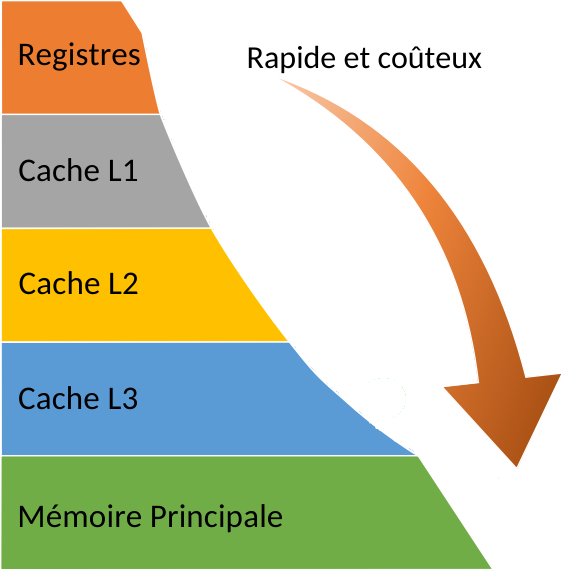
\includegraphics[width=0.5\linewidth]{schemas/hierarchieMemoire}
	\caption[hiérarchie mémoire multic\oe{}ur]{Schéma des types de mémoire intégrées selon leur taille et coût}
	\label{fig:hierarchiememoire}
\end{figure}

Plusieurs intermédiaire ont été mis en place entre ces deux types de mémoire. Il s'agit typiquement de trois niveaux de cache L1, L2 et L3. Les caches L1 et L2 sont dits non partagés, c'est-à-dire propres à chaque c\oe{}ur. Le cache L3 est partagé entre les c\oe{}urs. Ce dernier niveau est classiquement appelé LLC (\emph{Last Level Cache}) et donne la limite entre les espaces mémoire limités en cache avec des accès rapides d'une part et la mémoire principale qui va provoquer de grands ralentissements d'autre part. La gestion du contenu de ces caches (en lecture et écriture) est géré par une politique d'accès mémoire. Cette politique est essentielle à un usage efficace des caches du fait de leur espace limité qui demande à faire des choix sur son usage. Cela est peu documenté par les constructeurs,  et chacun aura sa façon de faire. 

La méthode de base la plus répandue étant empirique, par principe de localité temporelle~\cite{durrieu2014predictable} et spatiale~\cite{wilkes1965slave}. On considère que plus une donnée a été récemment accédée, plus elle a de chance d'être à nouveau utilisée. De même si une donnée est sollicitée, alors les données proches spatialement ont aussi plus de chance d'être utilisées. 
Nous n'iront pas plus dans les détails sur les politiques de gestion d'accès à la mémoire. Il faut garder en mémoire qu'elle est plutôt subie par les industriels qui intègrent le matériel dans leurs systèmes. Pour un processeur donné on aura certaines performances de calcul et accès mémoire, et il faudra mettre en comparaison les performances "par défaut" d'un logiciel sur une architecture donnée face au même système mais avec des surcouches de gestion du logiciel apportées par l'intégrateur. Un exemple de processeur multi-c\oe{}ur avec hiérarchie mémoire est indiqué en figure \ref{fig:multicoeurintel}. On y retrouve plusieurs c\oe{}urs, ayant chacun leur propre niveau de cache L1 et L2. Le Niveau de cache L3 étant partagé entre tous les c\oe{}urs. 
\begin{figure}
	\centering
	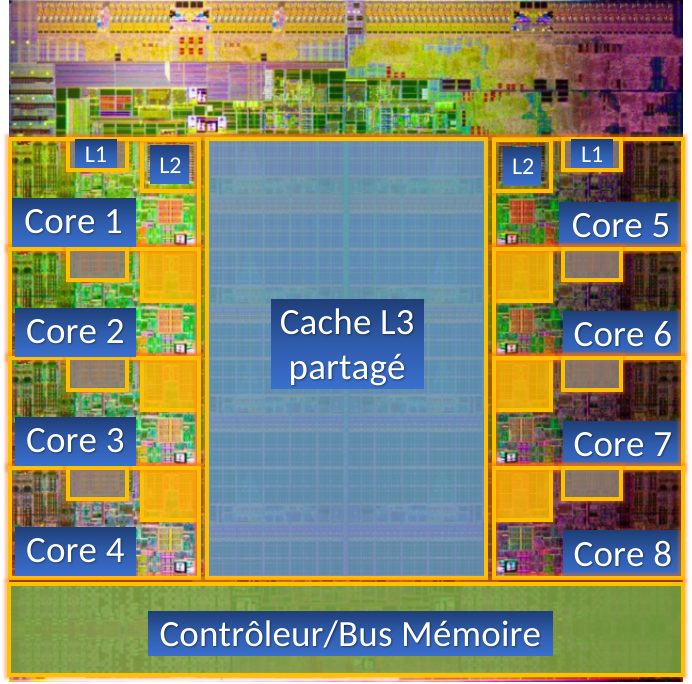
\includegraphics[width=0.5\linewidth]{schemas/multicoeurIntel}
	\caption[multicoeur]{Exemple d'architecture multicoeur - Processeur Intel I7}
	\label{fig:multicoeurintel}
\end{figure}



\subsection{Mono/Multi/Many Cores et GPU}
\subsection{Architectures mémoires, cas des multi-c\oe{}urs}
\subsection{Risques d'interférences}


\section{Enjeux des usages des multi-c\oe{}urs avec contraintes temporelles}
\subsection{Problématique :  criticité multiple : comment optimiser l'usage des ressources avec garanties temporelles}
